\section{Area-by-Area}
\label{sec:area-by-area}

In this section, each of the semantic areas introduced in Section \ref{subsec:semantic-areas} will be explored in depth and, in particular, the main elements that comprise it will be described. Bold font will be used to indicate classes, monospaced font for \acp{URI}, and italic font for properties. The prefixes in Table \ref{tab:ontopia-ontologies} will be used for \acp{URI}.

\subsection{Demographic Observations and Events}
\label{subsec:demographic-observations}

This semantic area is represented in Figure \ref{fig:demographic-sa}, and comprehends the classes and the properties that describe demographic observations and events for the domains of demographic statistics, civil status, tourism, events, schools, and organizations.

\begin{sidewaysfigure}[!ht]
  \centering
  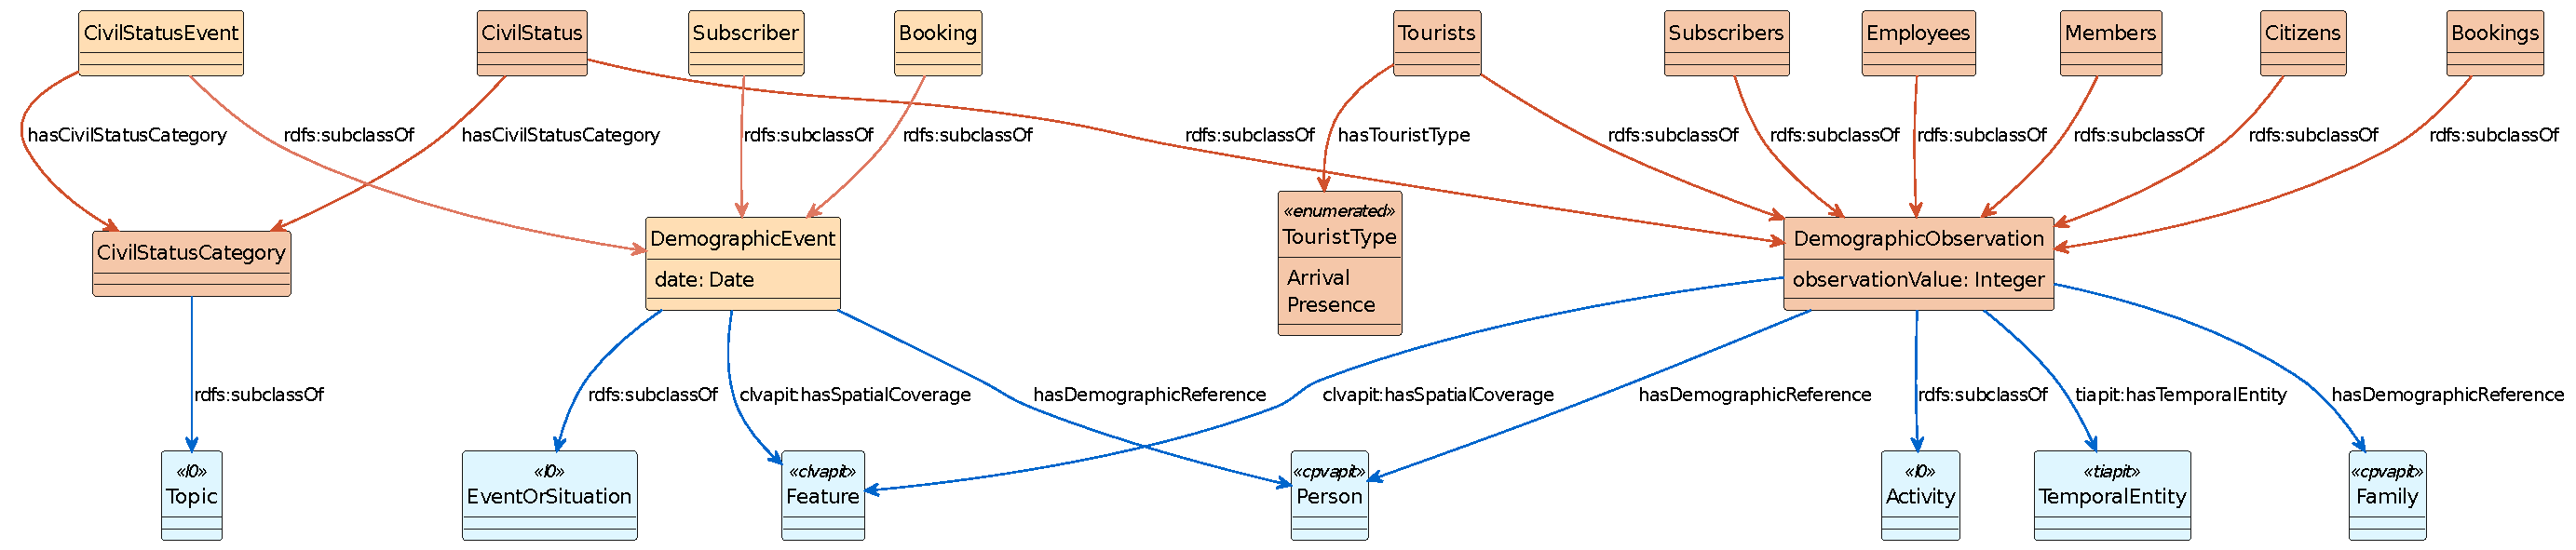
\includegraphics[width=\columnwidth]{images/ontoim/demographic}
  \caption{Demographic Observations and Events semantic area.}
  \label{fig:demographic-sa}
\end{sidewaysfigure}

There are two main classes in this area. The \textbf{Demographic Observation} class (\verb#:DemographicObservation#), and the \textbf{Demographic Event} (\verb#:DemographicEvent#) class. This makes it possible to represent data either in aggregate form (e.g., the number of marriages in a year) or, where possible, as individual events (e.g., a wedding occurred on a particular day).

The class \textbf{Demographic Observation}, which is a subclass of the \textbf{Activity} class (\verb#l0:Activity#) has the data property \textit{observationValue} (\verb#xsd:nonNegativeInteger#), which represents the quantity of the observation (e.g. the number of citizens). Through the properties \textit{hasTemporalEntity} and \textit{hasSpatialCoverage}, \textbf{DemographicObservation} is connected to \textbf{TemporalEntity} (\verb#tiapit:TemporalEntity#) and \textbf{Feature} (\verb#clvapit:Feature#) respectively. In this way it is possible to define the time and space to which the observation refers. To get more accurate statistics, it may be useful to distinguish observations by gender, citizenship or other characteristics. Instead of adding different properties for each of these characteristics, you can use the \textit{hasDemographicReference} property, which connects \textbf{DemographicObservation} to a \textbf{Person} (\verb#cpvapit:Person#) class or \textbf{Family} (\verb#cpvapit:Family#) class for observations about families. These classes then reference the observed characteristics.

Different type of observations are modeled using subclasses of the class \textbf{DemographicObservation}. The main subclasses are:

\begin{description}
  \item[Tourists]  (\verb#:Tourists#) To describe observations about the number of tourists. We can distinguish two type of observations about tourism: arrivals and presences. The \textit{hasTouristType} property connect \textbf{Tourists} to the enumerated class \textbf{TouristType} (\verb#TouristiType#), which can be \verb#:Arrival# or \verb#Presence#;
  \item[CivilStatus]  (\verb#:CivilStatus#) To describe the number of civil status events (e.g. births, deaths, marriages, \etc). The typology of the event is defined through the class \textbf{CivilStatusCategory} (\verb#:CivilStatusCategory#), connected by the property \textit{hasCivilStatusCategory}. The available categories are defined in a controlled vocabulary following the entries in the ISTAT D.7.A model\footnote{\url{https://purl.archive.org/istat-d7a-sona-2021}} of civil status statistics.
  \item[Subscribers] (\verb#:Subscribers#) This subclass is used to describe observations about subscribers to events, school, and courses.
\end{description}

The remaining subclasses, which doesn't have additional properties, are: \textbf{Employees} (\verb#:Employees#), \textbf{Members} (\verb#:Members#), \textbf{Citizens} (\verb#:Citizens#), and \textbf{Bookings} (\verb#:Bookings#). They describe respectively: (1) the number of employees that works in a organization; (2) the number of members of an association; (3) demographic observation on the population; (4) the number of bookings in a accommodation facility.

\paragraph*{}
The \textbf{DemographicEvent} class is similar to \textbf{DemographicObservation}, but, as said before, is used to represent singular events. It shares with the latter the \textit{hasDemographicReference} and \textit{hasSpatialCoverage} properties, but it has the property \textit{date}, which defines the date on which the event occurred. Different subclasses are used to model specific types of events. In particular, such subclasses are: (1) \textbf{CivilStatusEvent} (\verb#:CivilStatusEvent#), which is the equivalent of \textbf{CivilStats} for the observations; (2) \textbf{Subscriber} (\verb#:Subscriber#), to model a single registration to an event, school or course; (3) \textbf{Booking} (\verb#:Booking#), to describe a single reservation to an accommodation facility.

\subsection{Facilities and Cadastral Data}
\label{subsec:facilities}

Figure \ref{fig:facilities-sa} represent the semantic area of facilities and cadastral data, which are used to describe schools, hospitals, green zones \etc.

\begin{figure}[!ht]
  \centering
  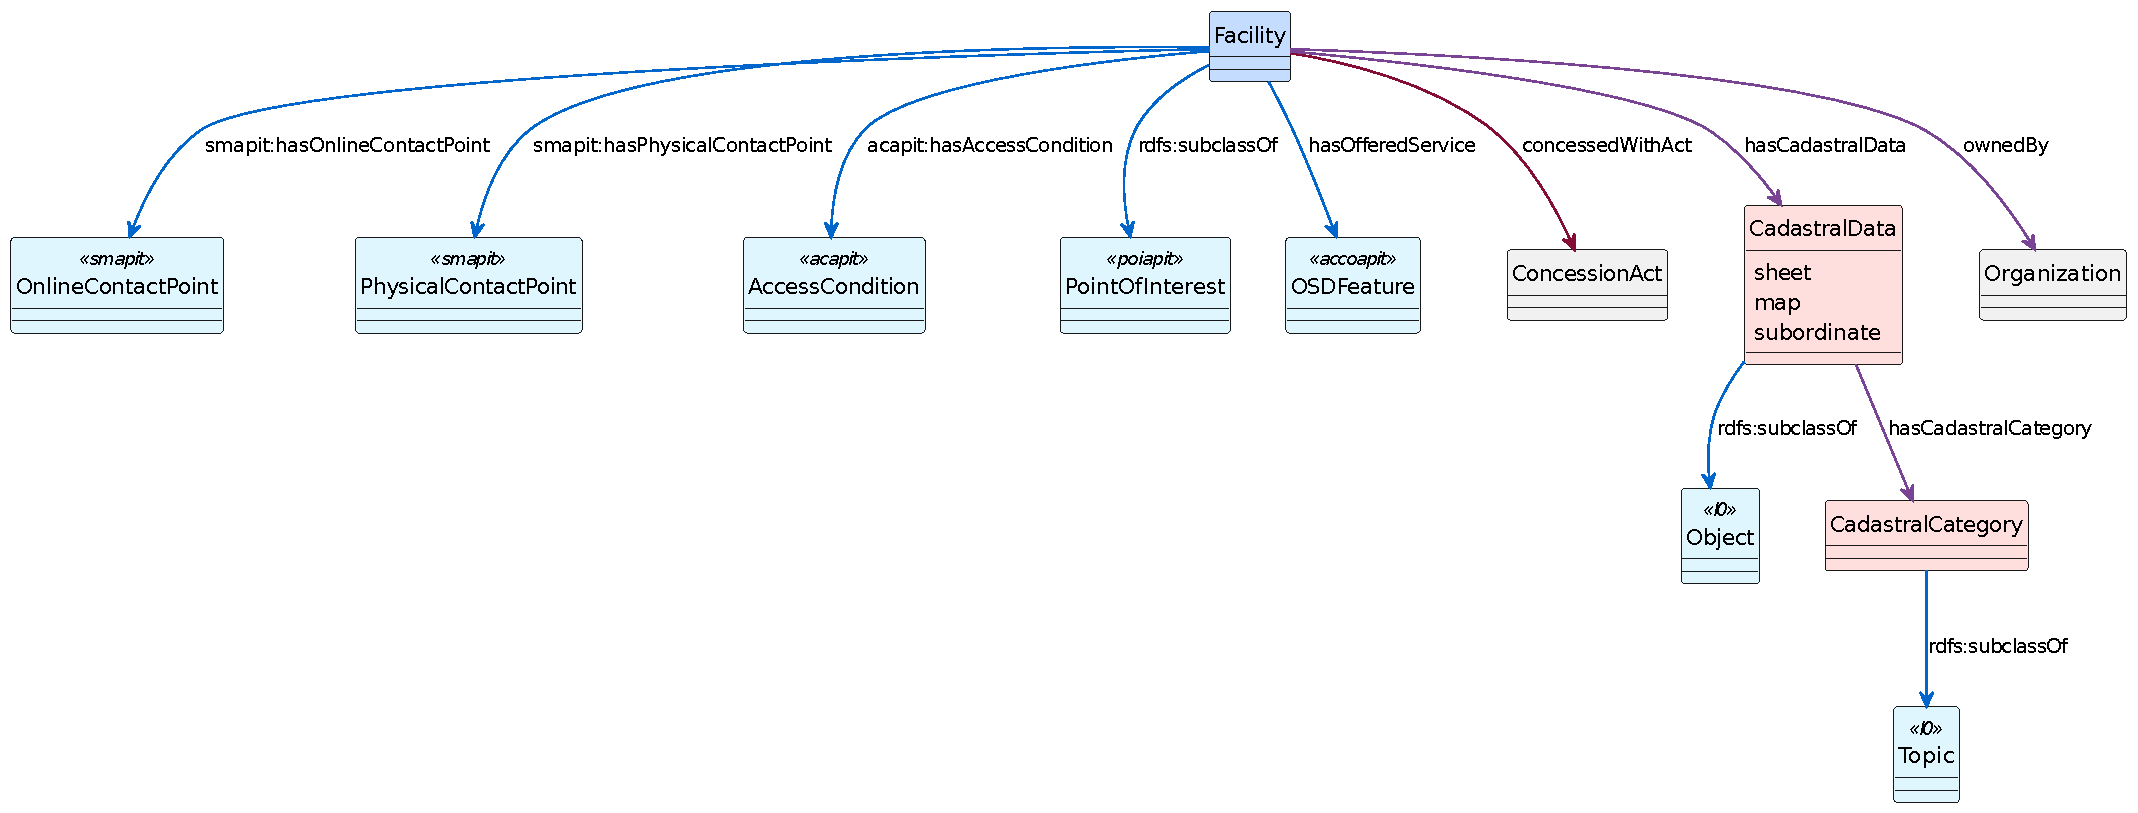
\includegraphics[width=\columnwidth]{images/ontoim/facilities}
  \caption{Facilities and Cadastral Data semantic area.}
  \label{fig:facilities-sa}
\end{figure}

The main class is \textbf{Facility} (\verb#:Facility#), which is a subclass of the \verb#POI-AP_IT#'s \textbf{PointOfInterest} class (\verb#poiapit:PointOfInterest#), and from which it inherits all the properties. The properties \textit{hasOnlineContactPoint}, \textit{hasPhysicalContactPoint}, and \textit{hasAccessConditions} connect the \textbf{Facility} class respectively to: (1) \textbf{OnlineContactPoint} (\verb#smapit:OnlineContactPoint#), which defines online contact points such as emails, social network usernames, websites, and telephones; (2) \textbf{PhysicalContactPoint} (\verb#smapit:PhysicalContactPoint#), which describes the address or the Point of Interest where the facility is located; (3) \textbf{AccessCondition} (\verb#acapit:AccessCondition#), which defines the facility opening hours. The \textbf{OSDFeature} class (\verb#accoapit:OSDFeature#) is connected through the property \textit{hasOfferedService}, and it is used to describe services and features that the facility offers (e.g. air conditioning, food service, parking, \etc).

A facility can be owned by an organization, but can be granted for use to another organization or to a person through a deed of grant. This situation is described by the property \textit{ownedBy}, which connect the facility to the \textbf{Organization} class that represents its owner; the property \textit{concessedWithAct} and the class \textbf{ConcessionAct} (\verb#:ConcessionAct#), which is described in Section \ref{subsec:transparency}.

\paragraph*{}
Finally, a facility is identified in the land registry by one or more cadastral data. The class \textbf{CadastralData} (\verb#:CadastralData#) stores this information, and it is connected to the \textbf{Facility} class through the \textit{hasCadastralData} property. A facility has also a cadastral category, defined by the class \textbf{CadastralCategory} (\verb#:CadastralCategory#). The elements of this class must be defined according to a controlled vocabulary that store the available cadastral categories.\footnote{\url{https://purl.archive.org/age-categorie-catastali}}

\subsection{Organizations and Associations}
\label{subsec:organizations-associations}

This semantic area is represented in Figure \ref{fig:organizations-sa}, and covers the domains of public and private organizations, and associations. The area was designed following the structure of the data provided by the Camera di Commercio.\footnote{\url{https://www.mn.camcom.gov.it/files/RegistroImprese/Legenda-elenchi.pdf}}

\begin{figure}[!ht]
  \centering
  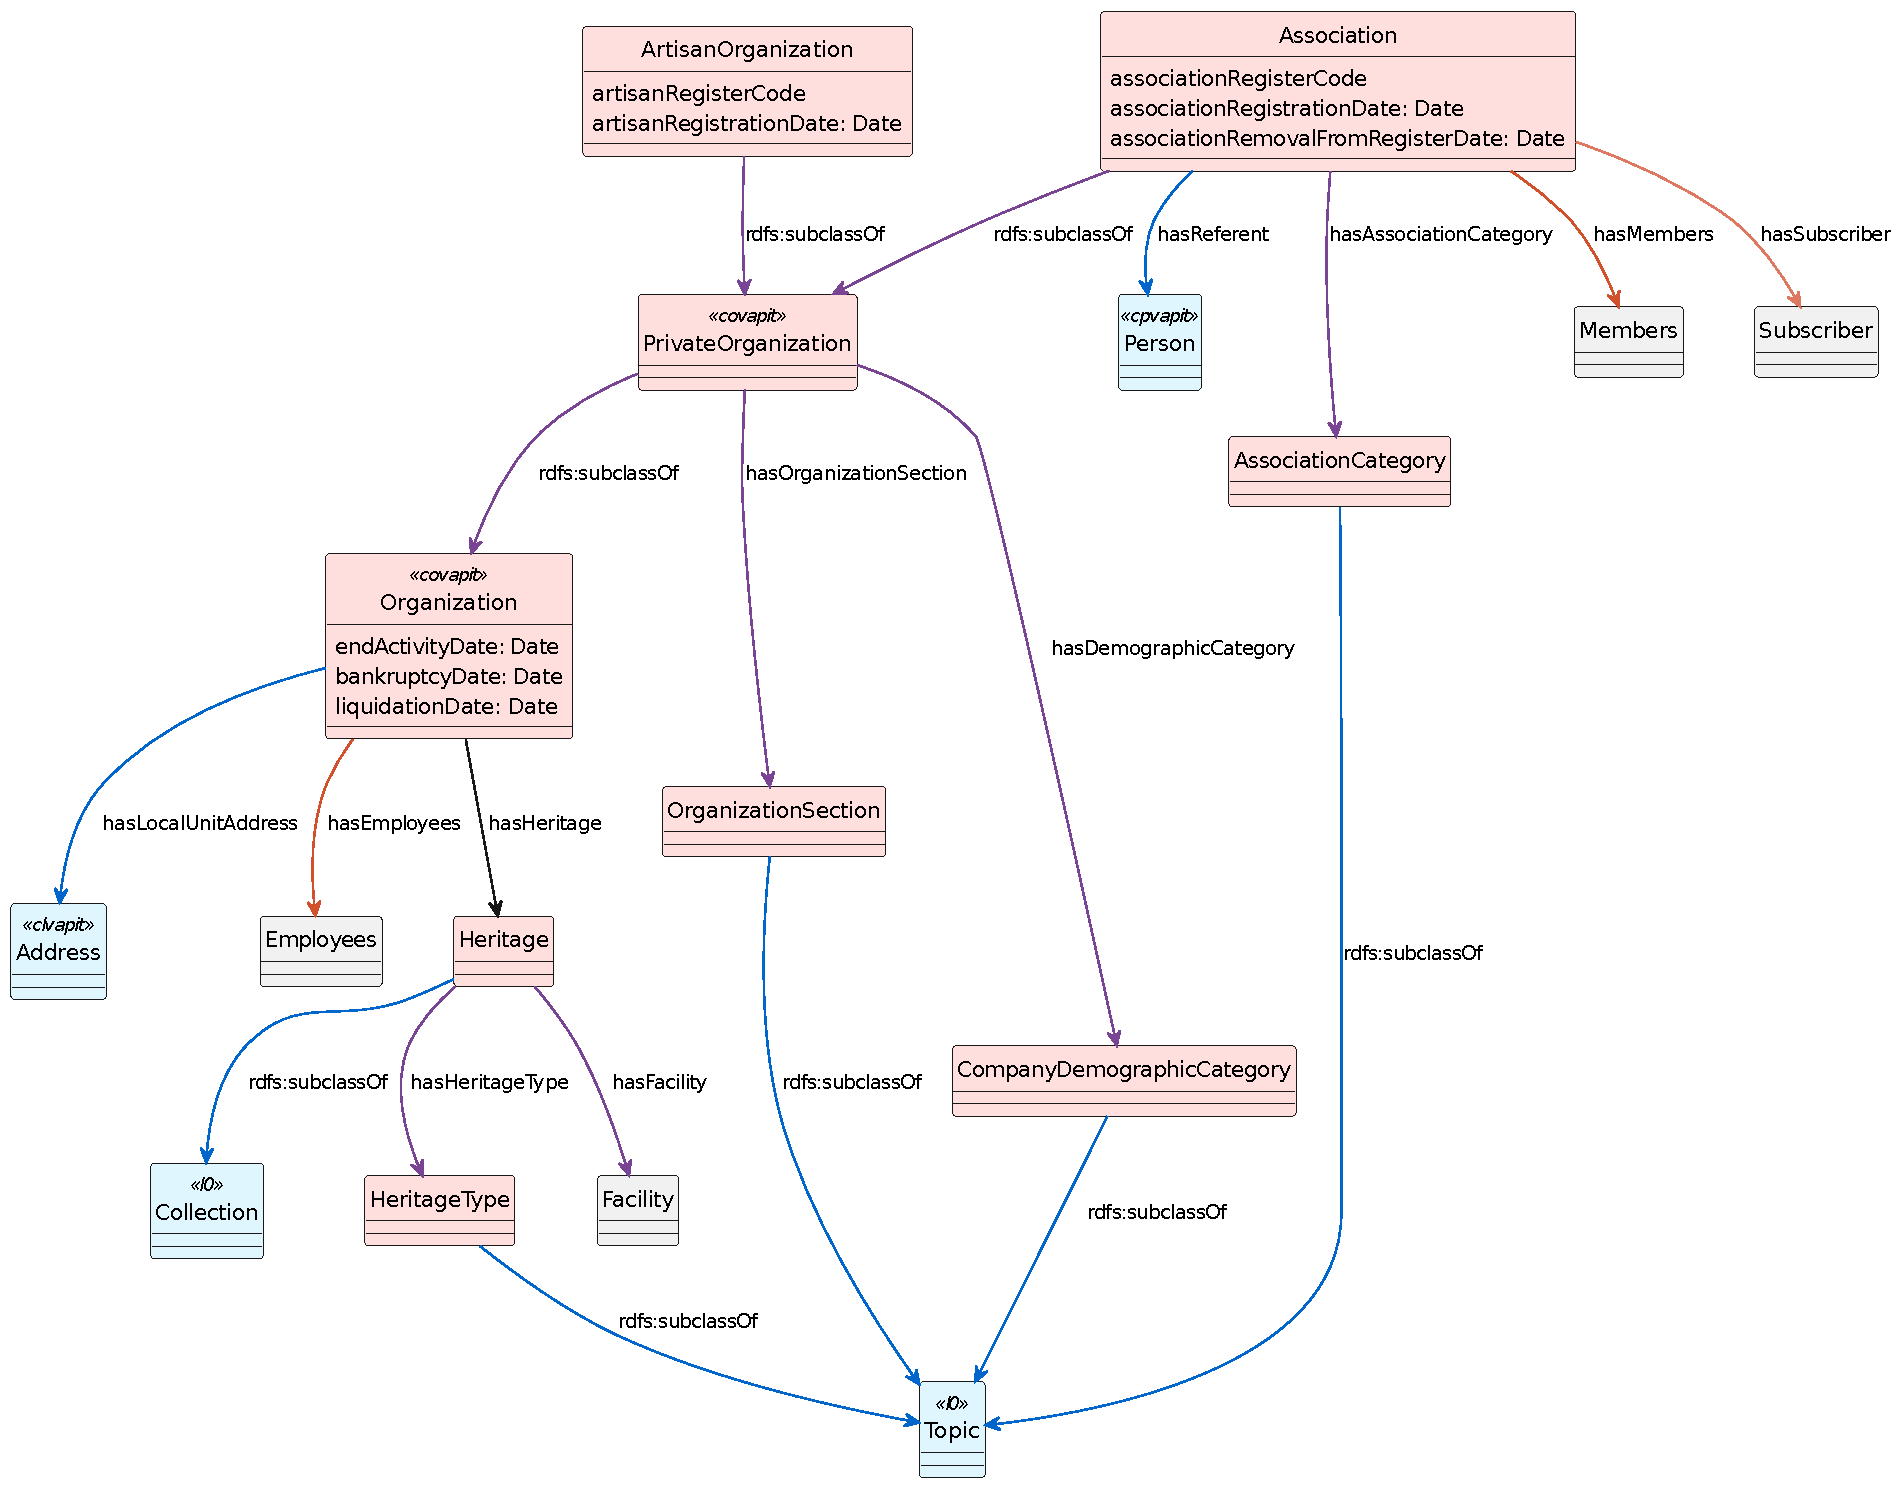
\includegraphics[width=\columnwidth]{images/ontoim/organizations}
  \caption{Organizations and Associations semantic area.}
  \label{fig:organizations-sa}
\end{figure}

Three data properties concerning events in the life cycle of an organization have been added to the \verb#COV-AP_IT#'s \textbf{Organization} class (\verb#covapit:Organization#). These properties, of type \verb#xsd:date#, are \textit{endActivityDate}, \textit{bankruptcyDate}, and \textit{liquidationDate}.

The property \textit{hasLocalUnitAddress} connects the \textbf{Organization} class to an \textbf{Address} class (\verb#clvapit:Address#), and it is used to store the addresses of one or more local units of the organization. It should also be specified that an organization may have its primary address in another city and a local unit in the municipality concerned. In that case, the Camera di Commercio provides only the address of the latter, specifying that it is a local unit.

An organization may also have real estate assets. Since there can be different types of heritage, such as unavailable heritage or state property, the structures owned by the organization are grouped, through the property \textit{hasFacility}, in the \textbf{Heritage} class (\verb#:Heritage#), to which its type defined by the \textbf{HeritageType} class (\verb#:HeritageType#) is linked, through the property \textit{hasHeritageType}, and whose elements are defined in a controlled vocabulary.

For what concern demographic observations, as specified in Section \ref{subsec:demographic-observations}, the \textbf{Employees} class describes the number of employees that works in the organization.

This semantic area also extends the \verb#COV-AP_IT#'s \textbf{PrivateOrganization} class (\verb#covapit:PrivateOrganization#), which is a subclass of an \textbf{Organization}. The property \textit{hasOrganizationSection} connect the company to the \textbf{OrganizationSection} class (\verb#:OrganizationSection#). The elements of this class are defined in a controlled vocabulary created from the sections provided by the Camera di Commercio. Another controlled vocabulary defines the elements that must be used for the \textbf{CompanyDemographicCategory} class (:CompanyDemographicCategory), which defines whether the enterprise is a youth, female or foreign enterprise. Finally, artisan organizations are described by the class \textbf{ArtisanOrganization} (\verb#:ArtisanOrganization#), which has the two data properties \textit{artisanRegisterCode} (\verb#rdfs:Literal#), which define the identifier of the organization in the register of artisans, and \textit{artisanRegistrationDate} (\verb#xsd:date#), which define the date when the organization was registered.

\paragraph*{}
Associations are treated as private organizations. Indeed, the \textbf{Association} class (\verb#:Association#) is a subclass of the \textbf{PrivateOrganization} class. The data property \textit{associationRegisterCode} (\verb#rdfs:Literal#) defines the identifier of the association in the register of associations. The other two data properties, \textit{associationRegistrationDate}, and \textit{associationRemovalFromRegisterDate}, define the life cycle events for an association.
The class \textbf{AssociationCategory} (\verb#:AssociationCategory#), connected through the property \textit{hasAssociationCategory}, define the category of the association (such as ONLUS, cultural association, \etc). The elements of this class must be defined according to a controlled vocabulary.

Finally, as specified in Section \ref{subsec:demographic-observations}, the \textbf{Members} class is used to describe demographic observations on the members of the association, while the \textbf{Subscriber} class is used to describe singular membership events.

\subsection{Transparency}
\label{subsec:transparency}

This semantic area contains classes that extend the \verb#Transparency-AP_IT# ontology for transparency obligation. These classes are graphically represented in Figure \ref{fig:transparency-sa}.

\begin{figure}[!ht]
  \centering
  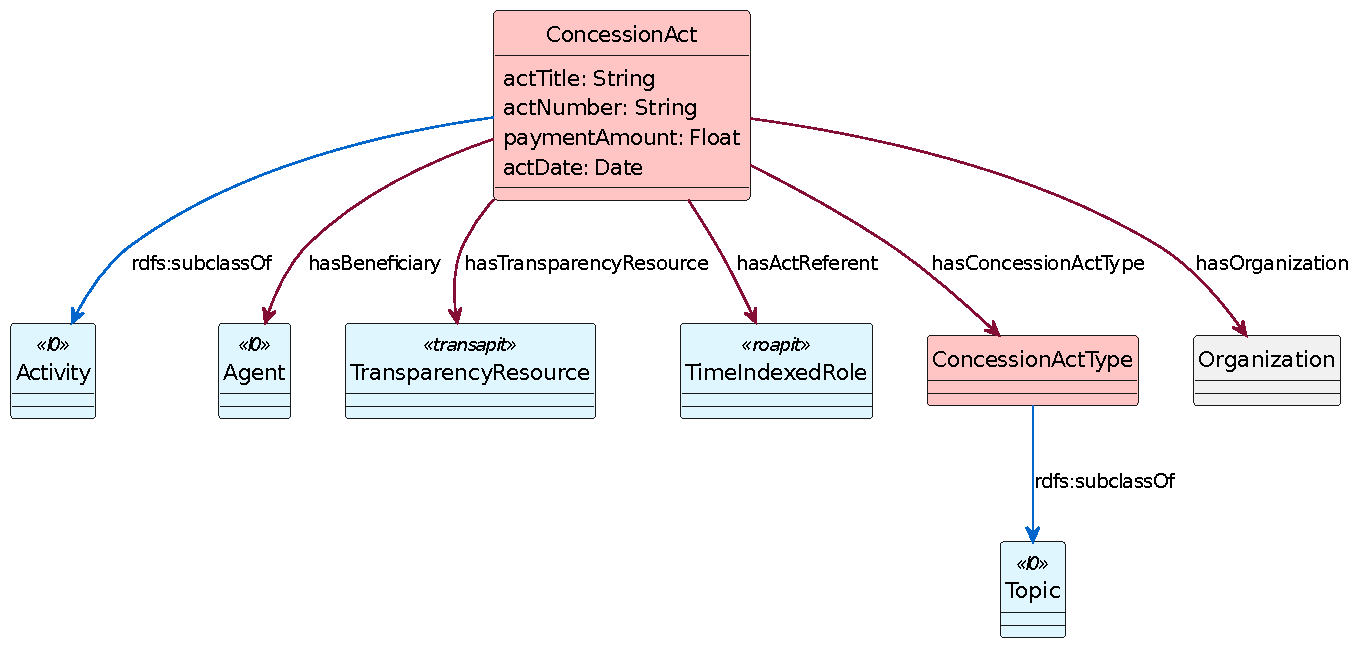
\includegraphics[width=\columnwidth]{images/ontoim/transparency}
  \caption{Transparency semantic area.}
  \label{fig:transparency-sa}
\end{figure}

The main class is \textbf{ConcessionAct} (\verb#:ConcessionAct#), which defines a deed of concession from an organization to another organization or person, and it is used either to grant the management of a facility, or to send a payment. The data properties of the \textbf{ConcessionAct} class are: (1) \textit{actTitle} (\verb#xsd:string#), which defines the title of the act; (2) \textit{actNumber} (\verb#xsd:string#), which defines the code number of the act; (3) \textit{paymentAmount} (\verb#xsd:float#), which defines the amount of the payment; (4) \textit{actDate} (\verb#xsd:date#), which defines the date of the act.

The \textit{hasBeneficiary} property connects the \textbf{ConcessionAct} to the \textbf{Agent} class (\verb#l0:Agent#), which can be both an organization or a person. The organization that sign the concession act is connected by the \textit{hasOrganization} property.

The signed document of the concession act can be stored as a \textbf{TransparencyResource} element (\verb#transapit:TransparencyResource#). 

The referent of the organization that sign the concession act is defined by a \textbf{TimeIndexedRole} class (roapit:TimeIndexedRole) through the property \textit{hasActReferent}.

Finally, the typology of the concession act is defined by the \textbf{ConcessionActType} class (\verb#:ConcessionActType#), whose elements are defined in a controlled vocabulary.

\subsection{Roads and Traffic}
\label{subsec:roads-traffic}

This semantic area, which is represented in \ref{fig:roads-sa}, extends the OntoPiA ontology regarding the traffics flow observations, and contains classes that describe the road signals and the road accidents.

\begin{sidewaysfigure}[!ht]
  \centering
  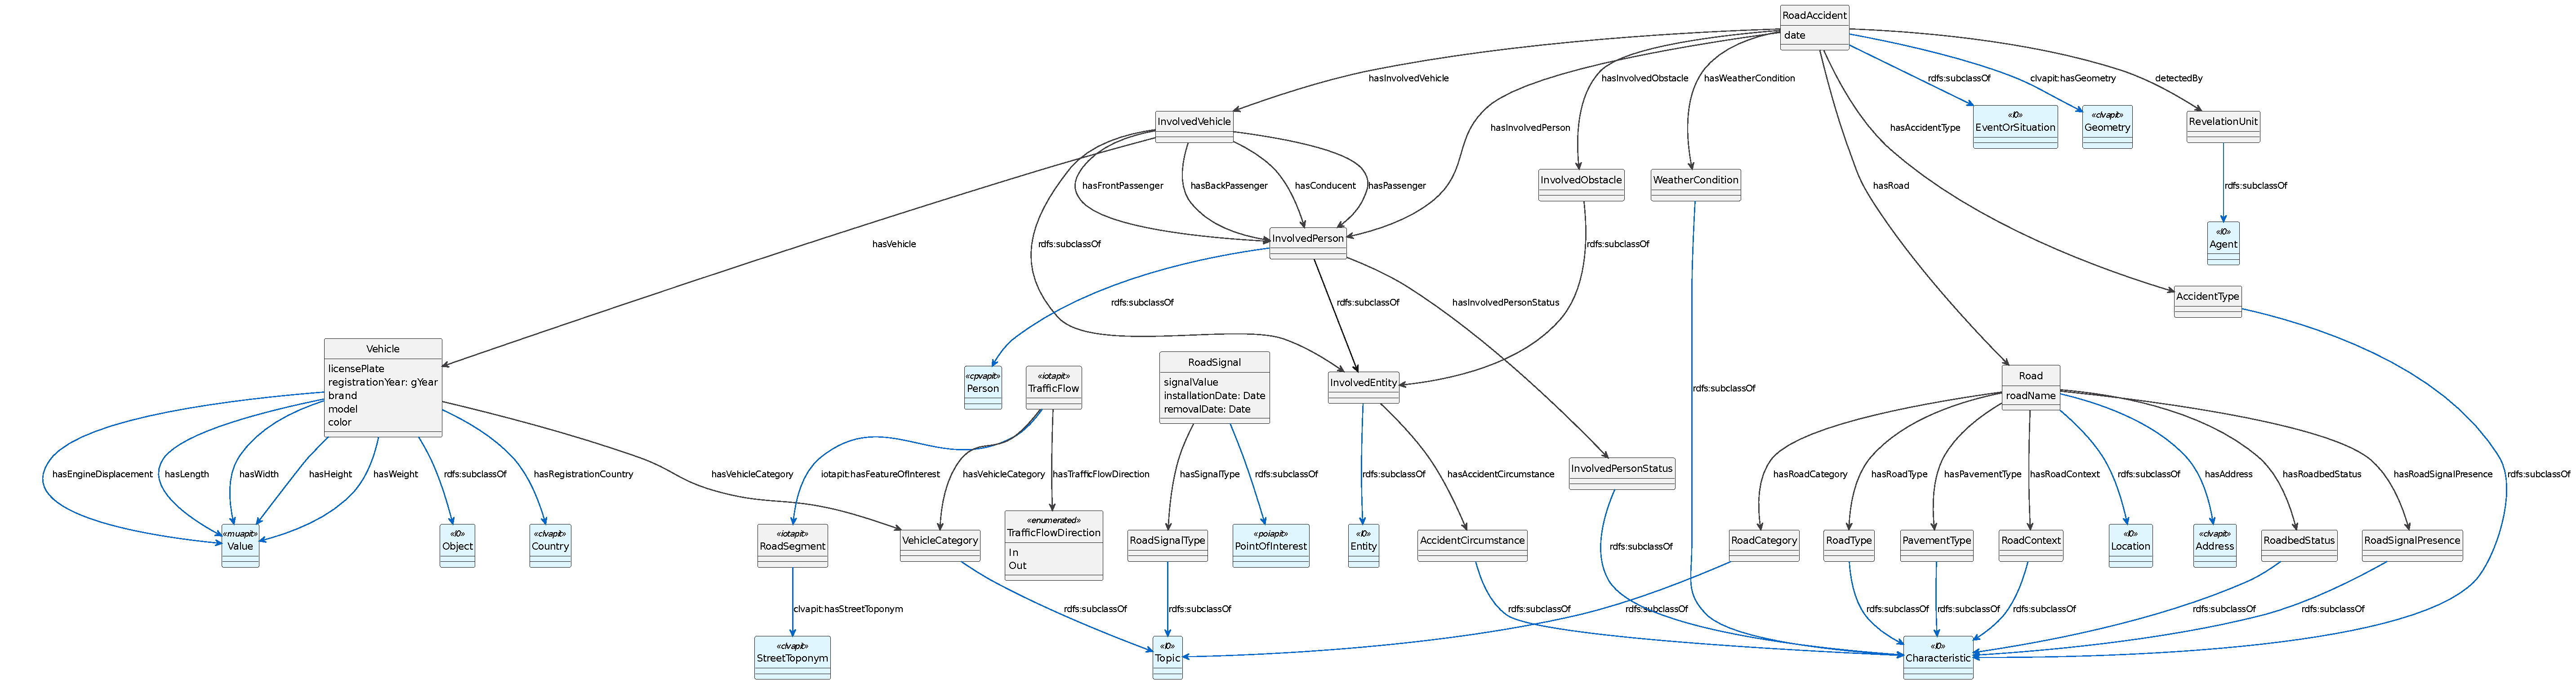
\includegraphics[width=\columnwidth]{images/ontoim/roads}
  \caption{Roads and Traffic semantic area.}
  \label{fig:roads-sa}
\end{sidewaysfigure}

For what concerns the traffic flow observations, the \verb#IOT-AP_IT#'s \textbf{TrafficFlow} class (\verb#ioapit:TrafficFlow#) is connected through the property \textit{hasTrafficFlowDirection} to the \textbf{TrafficFlowDirection} class (\verb#:TrafficFlowDirection#). This class represents the direction of the flow respect to the sensor, and is thus an enumerated class that can have individual \verb#:In# or individual \verb#:Out# as its elements. The \textbf{RoadSegment} (\verb#:RoadSegment#) class, which define the feature of interest for the observation, is connected through the property \textit{hasStreetToponym} to the name of the road observed, represented by the \textbf{StreetToponym} class (\verb#clvapit:StreetToponym#). Finally, the observations can be enriched with the category of vehicle observed. This can be done through the property \textit{hasVehicleCategory} that connects \textbf{TrafficFlow} to the \textbf{VehicleCategory} class (\verb#:VehicleCategory#). The elements of this class are in a controlled vocabulary, whose elements are defined following the road code classification.\footnote{\url{https://www.polizialocaleterredifrontiera.com/codice-della-strada/veicoli/}}

\paragraph*{}
It is also useful for a city to keep track of the status and location of street signs to aid their maintenance. The class \textbf{RoadSignal} (\verb#RoadSignal#) describes a street sign, and is a subclass of the \textbf{PointOfInterest} class (\verb#poiapit:PointOfInterest#). In addition to those inherited from the \textbf{PointOfInterest} class (such as the location), the \textbf{RoadSignal} class has three more data properties: (1) \textit{installationDate} (\verb#xsd:date#), which defines the date when the signal was installed; (2) \textit{removalDate} (\verb#xsd:date#), which defines the date when the signal was removed; (3) \textit{signalValue}, which defines the value on the signal (e.g. the speed for a speed limit signal). The typology of the road signal is defined through the property \textit{hasSignalType}, which connects it to the class \textbf{RoadSignalType} (\verb#:RoadSignalType#). The elements of this class are defined in a controlled vocabulary generated from the list of road signs in Italy.\footnote{\url{https://it.wikipedia.org/wiki/Segnaletica_stradale_in_Italia}}

\paragraph*{}
The last subarea is dedicated to road accidents, and was developed following the ISTAT model used to collect road accidents, both to design the ontology and to define the controlled vocabularies.\footnote{\url{https://purl.archive.org/istat-incidenti-stradali-2018}}

The main class is \textbf{RoadAccident} (\verb#:RoadAccident#), which is a subclass of \verb#L0#'s \textbf{EventOrSituation} (\verb#l0:EventOrSituation#). The date and time when the incident occurred are defined by the data property \textit{date} (\verb#xsd:dateTime#). The \textbf{Geometry} class (\verb#clvapit:Geometry#) describe the geographical location of the accident.

The property \textit{detectedBy} connects \textbf{RoadAccident} with the class \textbf{RelevationUnit} (\verb#:RelevationUnit#), defining who recorded the incident (e.g., police, carabinieri, \etc). The elements of the latter class are defined in a controlled vocabulary. The class \textbf{AccidentType} (\verb#:AccidentType#) defines the nature of the accident (e.g. head-on collision, pedestrian investment, \etc), and its elements are also defined in a controlled vocabulary. Another class whose elements are defined in a controlled vocabulary is \textbf{WeatherCondition} (\verb#:WeatherCondition#), which defines the weather conditions at the time of the accident.

The \textbf{Road} (\verb#:Road#) class is used to store information about the road and its status at the time of the accident. The address where the location happened is defined by the \textbf{Address} class (\verb#clvapit:Address#) through the property \textit{hasAddress}. Then, there are several classes that defines the context and the status of the road during the accident. The elements of these classes must all be defined according to the relative controlled vocabularies. Such classes are:

\begin{description}
  \item[RoadCategory] (\verb#:RoadCategory#), which defines whether the road is a municipal road, a state road, a highway, \etc;
  \item[RoadType] (\verb#:RoadType#), which defines whether the road is single- or multi-lane or one-way;
  \item[PavementType] (\verb#:PavementType#), which defines whether the road is paved or uneven;
  \item[RoadContext] (\verb#:RoadContext#), which defines whether the accident occurred at an intersection, traffic circle, on a straight road, \etc;
  \item[RoadbedStatus] (\verb#:RoadbedStatus#), which defines the status of the roadbed (e.g. dry, wet, frozen, \etc);
  \item[RoadSignalPresence] (\verb#:RoadSignalPresence#), which defines whether the road signals are present or not, or what type of signals are present.
\end{description}

Finally, there are some classes that describe the entities involved (obstacles, persons, vehicles) in the accident. These entities are described by the class \textbf{InvolvedEntity} (\verb#:InvolvedEntity#). The property \textit{hasAccidentCirumstance} connects this class to the \textbf{AccidentCircumstance} class (\verb#:AccidentCircumstance#), which defines what the entity involved was doing during the accident (e.g., the pedestrian was crossing the street, or the car was proceeding at high speed). The elements of this class are defined in a controlled vocabulary. To define whether the entity is a vehicle, an obstacle, or a person, the \textbf{InvolvedEntity} class has three subclasses: \textbf{InvolvedVehicle} (\verb#:InvolvedVehicle#), \textbf{InvolvedPerson} (\verb#:InvolvedPerson#), and \textbf{InvolvedObstacle} (\verb#:InvolvedObstacle#). The \textbf{InvolvedPerson} class inherits also the properties of the \verb#CPV-AP_IT#'s \textbf{Person} class (\verb#cpvapit:Person#), so it is possible to define the sex and age of the person involved. The status of the person involved (e.g. wounded, uninjured, dead, \etc) in the accident is described using the class \textbf{InvolvedPersonStatus} (\verb#:InvolvedPersonStatus#), whose elements are defined in a controlled vocabulary. For what concerns the vehicle, the class \textbf{InvolvedVehicle} has the properties \textit{hasFrontPassenger}, \textit{hasBackPassenger}, and \textit{hasConducent}, which are sub-properties of \textit{hasConducent}, and defines the person involved that was inside the vehicle. The \textbf{InvolvedVehicle} is also a subclass of the \textbf{Vehicle} class (\verb#:Vehicle#). This class, which represents a vehicle, has the data properties \textit{licensePlate} (\verb#xsd:string#), \textit{registrationYear} (\verb#xsd:gYear#), \textit{brand}, \textit{model}, and \textit{color}, which defines the characteristics of the vehicle. The properties \textit{hasEngineDisplacement}, \textit{hasLength}, \textit{hasWidth}, \textit{hasHeight}, and \textit{hasHeight} are used to describe the sizes of the vehicle, using the class \textbf{Value} (\verb#muapit:Value#). The category of the vehicle is described by the \textbf{VehicleCategory} class. The registration country is defined through the property \textit{hasRegistrationCountry}, which connects the \textbf{Vehicle} class to the \textbf{Country} class (\verb#clvapit:Country#).

Note that it was still chosen to include properties that in the Open Data environment would not be used for privacy reasons (e.g., the license plate or name of the people involved). This is because in this way the ontology can also be used internally to describe traffic accidents using Linked Data.

\subsection{Schools}
\label{subsec:schools}

The classes of this area describes the school, comprehensive institutes, and courses organized by schools. It should also be specified that in this ontology schools also include training institutions, music schools, sports associations, popular universities, \etc. Figure \ref{fig:schools-sa} shows the graphical representation of these classes.

\begin{sidewaysfigure}[!ht]
  \centering
  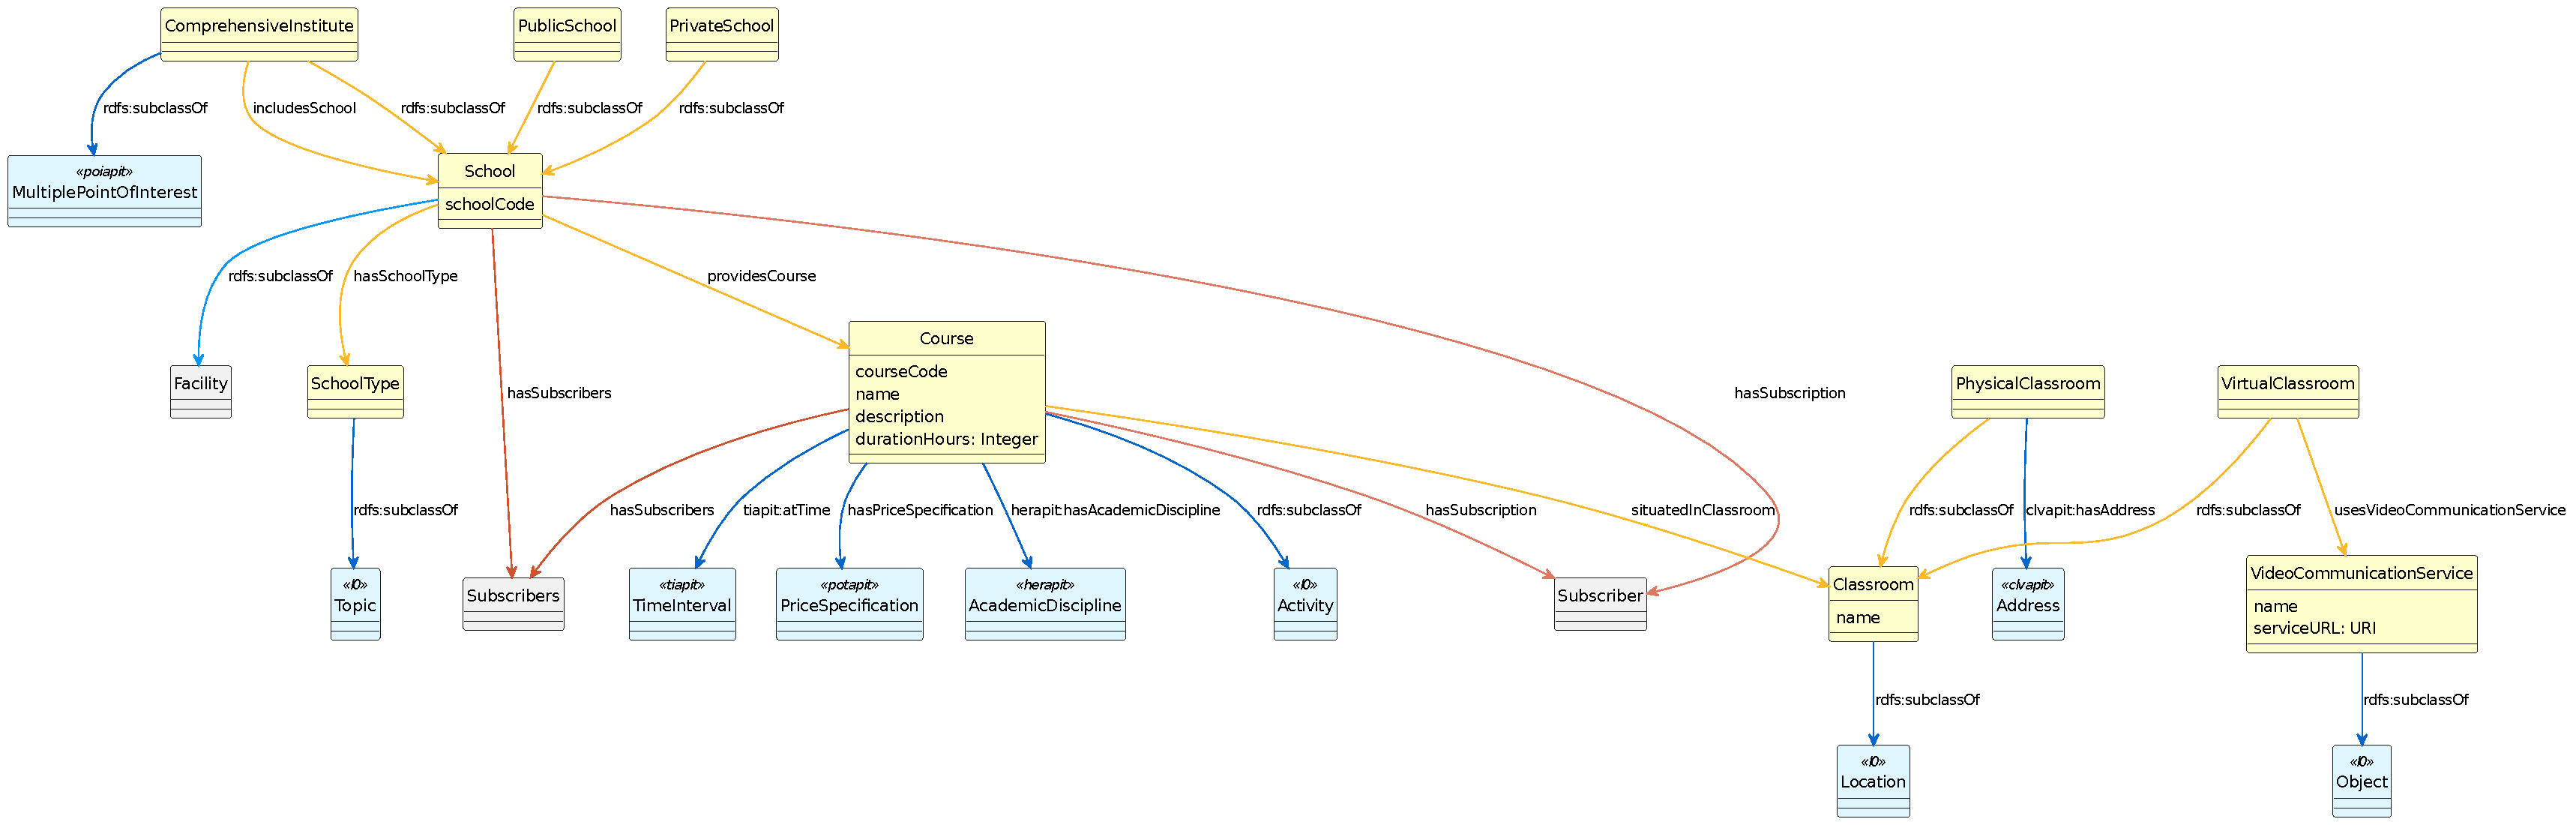
\includegraphics[width=\columnwidth]{images/ontoim/schools}
  \caption{Schools semantic area.}
  \label{fig:schools-sa}
\end{sidewaysfigure}

For what concern schools, the class \textbf{School} (\verb#:School#) is the core part of the area, and it inherits the properties from the \textbf{Facility} class. The data property \textit{schoolCode} represents the MIUR\footnote{\url{https://www.miur.gov.it/}} identifier for the school. The class \textbf{SchoolType} (\verb#:SchoolType#) defines the typology of the school (e.g. primary school, high school, \etc) and its elements must be defined according to a controlled vocabulary. The subclasses \textbf{PublicSchool} (\verb#:PublicSchool#), and \textbf{PrivateSchool} (\verb#:PrivateSchool#) are used to distinguish private and public schools. In Italy, schools are part of comprehensive schools. This situation is described by the \textbf{ComprehensiveInstitute} class (\verb#:ComprehensiveInstitute#), and the property \textit{includesSchool}, which links comprehensive institutes to the schools they include.

As said in Section \ref{subsec:demographic-observations}, the classes \textbf{Subscribers} and \textbf{Subscriber} are used to describe demographic observations on schoolchildren and enrollment events.

\paragraph*{}
For what concern courses, the core class of this subarea is \textbf{Course} (\verb#:Course#). The main information of the course are defined by the data properties \textit{courseCode}, which is the identifier of the course, \textit{name}, \textit{description}, \textit{durationHours}, and by the properties: (1) \textit{atTime}, which connects it to a \textbf{TimeInterval} class (\verb#tiapit:TimeInterval#) to define the period in which the course is provided; (2) \textit{hasPriceSpecification}, which connects \textbf{Course} to the class \textbf{PriceSpecification} (\verb#potapit:PriceSpecification#) to define the cost of the course, if any; (3) \textit{hasAcademicDiscipline}, which connects the \textbf{Course} class to the \textbf{AcademicDiscipline} class (\verb#:herapit:AcademicDiscipline#) to define the school discipline of the course.

The location (phisical or virtual) of the course is specified by the \textbf{Classroom} class (\verb#:Classroom#) through the property \textit{situatedInClassroom}. The subclass \textbf{PhysicalClassroom} (\verb#:PhysicalClassroom#) defines a physical classroom with an address defined by the class \textbf{Address}. On the other hand, if a course is provided using a video communication service, the classroom can be described as a \textbf{VirtualClassroom}, specifying also the service used through the class \textbf{VideoCommunicationService} (\verb#:VideoCommunicationService#), which describes the name of the service (e.g. Zoom, Google Meet), and its \ac{URL}.

\subsection{Green Zones and Plants}
\label{subsec:green-zones}

Figure \ref{fig:green-sa} represent this semantic area, which describes green zones (e.g. parks, flowerbeds, gardens), and plants.

\begin{figure}[!ht]
  \centering
  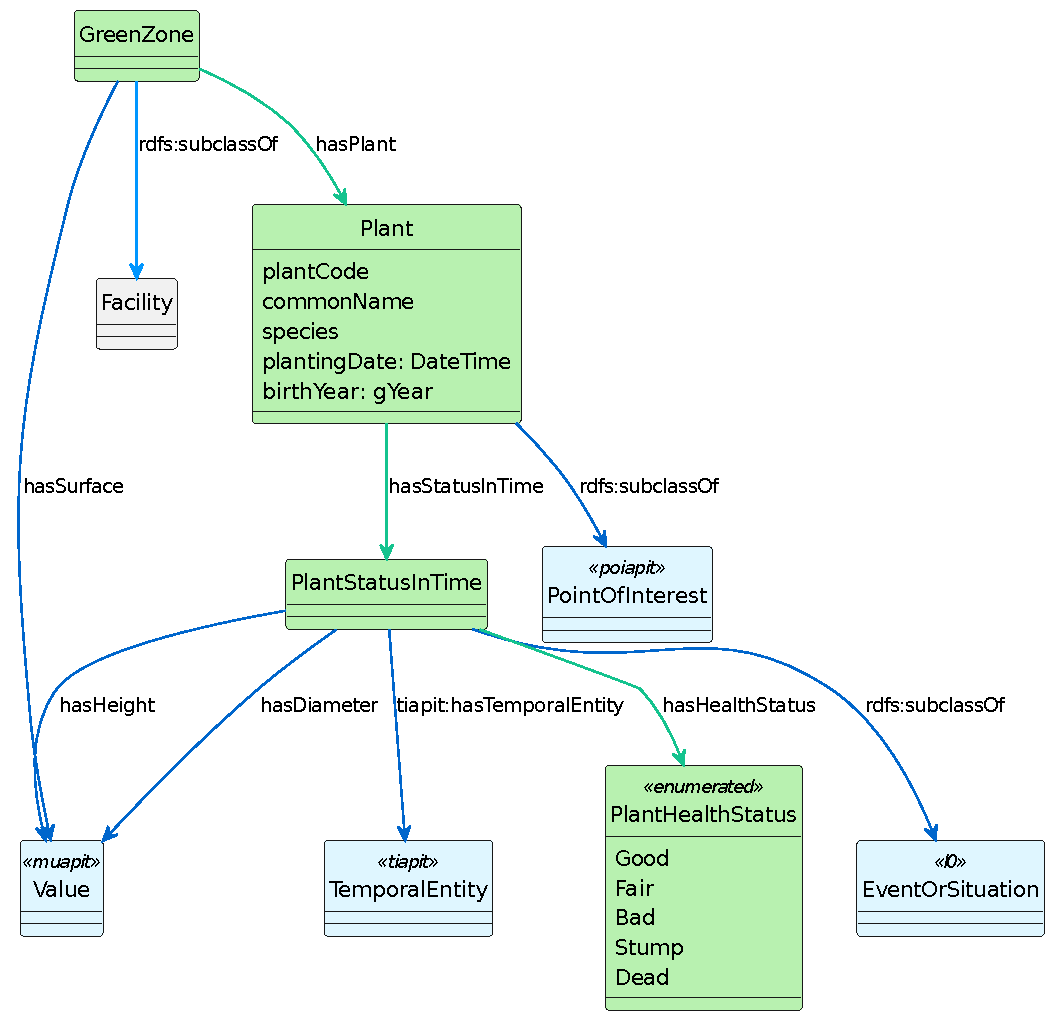
\includegraphics[width=0.6\columnwidth]{images/ontoim/green}
  \caption{Green Zones and Plants semantic area.}
  \label{fig:green-sa}
\end{figure}

A green zone is treated as a facility. Indeed, the class \textbf{GreenZone} (\verb#:GreenZone#) is a subclass of the class \textbf{Facility}, from which it inherits the properties. The size of the green zone is defined by the property \textit{hasSurface}, which connects the class to a \textbf{Value} class. A green area may have plants within it, so the \textit{hasPlant} property connects a green area with trees within it.

\paragraph*{}
The class \textbf{Plant} (\verb#:Plant#) contains the main immutable information about the plant: (1) \textit{plantCode} is the identifier; (2) \textit{commonName} the common name of the plant; (3) \textit{species} its species; (4) \textit{birtYear} (\verb#xsd:gYear#) the birth year; (5) \textit{plantingDate} (\verb#xsd:DateTime#) the planting date and time. It also inherits the properties from the class \textbf{PointOfInterest}, such as the geographical location of the plant.
Finally, it is useful to keep track of the state of the plant over time. The class \textbf{PlantStatusInTime} (\verb#:PlantStatusInTime#) do this, storing information about the dimensions of the plant, with the properties \textit{hasDiameter}, and \textit{hasHeight}, and the health status, using the enumerated class \textbf{PlantHealthStatus} (\verb#:PlantHealthStatus#).

\subsection{Hospitals}
\label{subsec:hospitals}

Figure \ref{fig:hospitals-sa} represents the hospitals.

\begin{figure}[!ht]
  \centering
  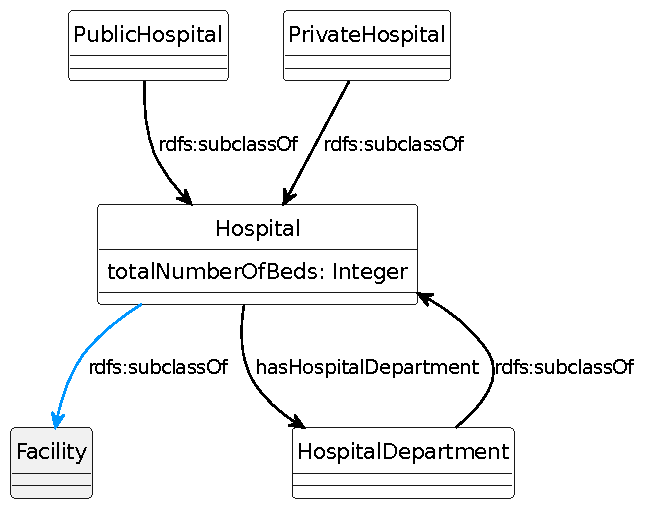
\includegraphics[width=0.5\columnwidth]{images/ontoim/hospitals}
  \caption{Hospitals semantic area.}
  \label{fig:hospitals-sa}
\end{figure}

The main class is \textbf{Hospital} (\verb#:Hospital#), which is a subclass of the \textbf{Facility} class, and form which it inherits the properties. The data property \textit{totalNumberOfBeds} defines the beds available in the hospital. The two subclasses \textbf{PublicHospital} (\verb#:PublicHospital#), and \textbf{PrivateHospital} (\verb#:PrivateHospital#) are used to specify the typology of the hospital.

Finally, as for school and comprehensive institutes, the class \textbf{HospitalDepartment} (\verb#:HospitalDepartment#) is treated as a hospital and describes the various departments into which a hospital is divided.

\subsection{Waste Production}
\label{subsec:waste-production}

This semantic area is represented in Figure \ref{fig:waste-sa}, and defines observations on waste production.

\begin{figure}[!ht]
  \centering
  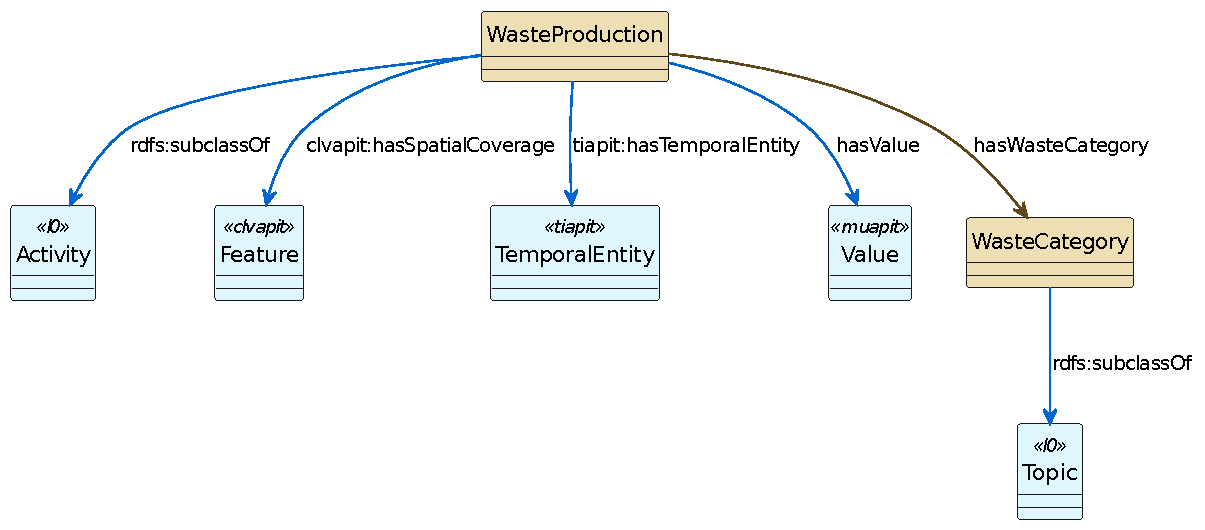
\includegraphics[width=\columnwidth]{images/ontoim/waste}
  \caption{Waste Production semantic area.}
  \label{fig:waste-sa}
\end{figure}

This semantic area is structured as demographic observation. The main class \textbf{WasteProduction} (\verb#:WasteProduction#) is connected to a \textbf{TemporalEntity} class, and a \textbf{Feature} class, which define the space and time to which the observation refers. The value of the observation is defined by the class \textbf{Value}, for which you can also define the unit of measurement (e.g. kg or t). To indicate an observation made on only one type of waste, the \textbf{WasteCategory} (\verb#:WasteCategory#) class can be used, whose elements are defined in a controlled vocabulary populated with the categories defined by ISPRA.\footnote{\url{https://www.isprambiente.gov.it/it}}